
\chapter{Graph Neural Networks as EPMs}
\label{ch:ch06:gnns_epms}
\providecommand{\gb}{GraphBench}

\begin{figure}[t]
	\centering
	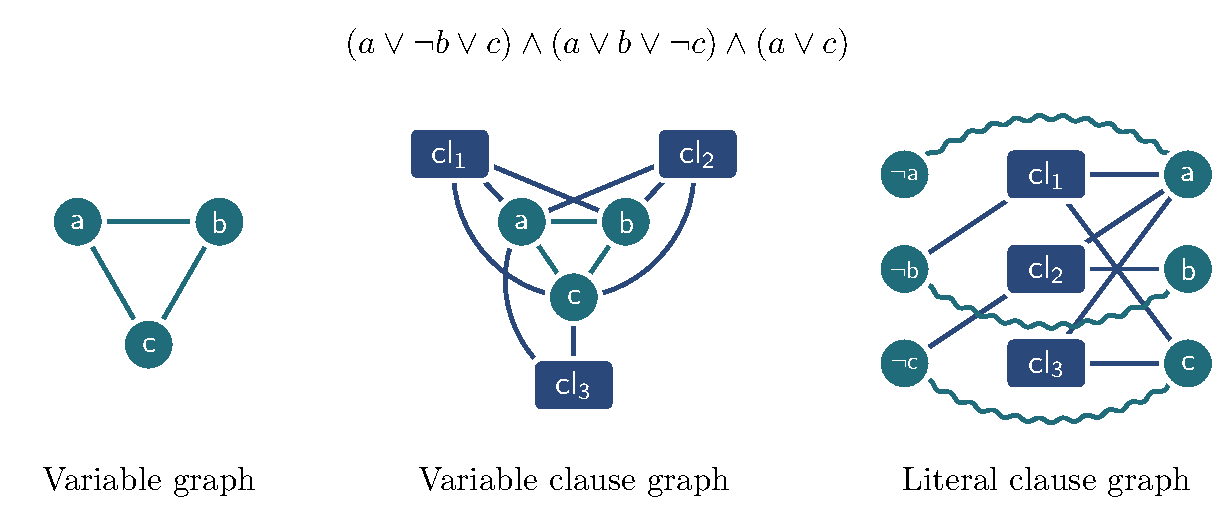
\includegraphics[width=0.75\textwidth]{figures/06/sat.pdf}
	\caption[Overview of SAT graph types]{Overview of the three graph types generated from a given \gls{sat} formula.
		\label{fig:ch06:sat}}
\end{figure}

\section{Introduction}

The \new{Boolean satisfiability problem} (\gls{sat}) is a central and longstanding \textsf{NP}-complete problem~\citep{Karp72,BieEtAl21b}. It asks whether there exists a truth assignment that satisfies a Boolean formula $\varphi$ over variables $v_1,\ldots,v_r$, typically expressed in \new{conjunctive normal form} (\gls{cnf}):
\begin{equation*}
	\varphi = \bigwedge_{i=1}^n c_i, \quad \text{where each } c_i = \bigvee_{j=1}^{m_i} l_{i, j}.
\end{equation*}
Here, each $l_{i,j}$ is a literal, i.e., either a variable $v_p$ or its negation $\lnot v_p$. The task is to decide whether there exists an assignment $a$ such that $\varphi(a) = \text{true}$. \Gls{sat} is of significant theoretical importance as one of the first problems proven \textsf{NP}-complete~\citep{Cook71}, and it underpins numerous practical applications in hardware and software verification~\citep{BieEtAl09}, automated planning~\citep{KauSel96}, and operations research~\citep{GomEtAl08}. Its significance has led to the development of a wide range of solvers, systematically benchmarked in annual \gls{sat} competitions (e.g.,~\citep{FroEtAl21,BalEtAl17,HeuEtAl19}). A key property of modern \gls{sat} solvers is \textit{performance complementarity}---no single solver dominates across all instances. This motivates the study of \emph{algorithm selection}~\citep{Rice76b,XuEtAl08b}, where the aim is to choose the most effective solver for a given instance. \new{Empirical performance prediction} is a closely related problem, which seeks to forecast the computation time (or another performance metric) of a solver on a given instance. Such predictions can support algorithm selection, configuration, scheduling, and explainability~\citep{HutEtAl14c}. State-of-the-art methods for algorithm selection and performance prediction rely on \textit{hand-crafted features} extracted from \gls{sat} instances. The most widely adopted feature set is that of the \textsc{SATzilla} family of algorithm selectors~\citep{NudEtAl04b,HutEtAl14c,ShaHoo24b}. These features include basic structural properties (e.g., number of clauses and variables), graph-based descriptors derived from instance structure, and probing features obtained by briefly running a solver to collect computation-time statistics. Machine learning models---most often tabular models---are then trained on these features for prediction or selection tasks.

\Gls{sat} instances can be naturally represented as graphs, reflecting their permutation-invariant structure that arises from the commutativity and associativity of logical conjunction and disjunction. Indeed, many of the hand-crafted \textsc{SATzilla} features are derived from such graph representations, including the
\begin{itemize}
	\item \new{Variable-clause graph}: a bipartite, undirected graph with a node for each variable $v$ and each clause $c$, where an edge connects a variable to a clause if and only if the variable appears in that clause.

	\item \new{Variable graph}: an undirected graph with one node per variable, where two variables $v_i$ and $v_j$ are connected if they co-occur in at least one clause.

	\item \new{Clause graph}: an undirected graph with one node per clause, where two clauses $c_i$ and $c_j$ are connected if they share at least one negated literal.
\end{itemize}

\textsc{SATzilla} extracts statistical properties of these graphs---such as mean degree, coefficient of variation, clustering coefficient, and graph diameter---and uses them as features for downstream learning tasks.

\section{Related work}

Several studies have explored the use of \glspl{gnn} or MPNNs to predict the satisfiability of a formula, e.g.,~\citet{SelEtAl19}. Some of this work employs an additional representation, the \new{literal-clause graph}, a bipartite graph with one node per literal (a variable or its negation) and one node per clause, with edges linking literals to the clauses they appear in. However, many such approaches are \emph{unsound}---they can produce incorrect results---or cannot guarantee valid satisfying assignments or proofs of unsatisfiability, limiting their practical usefulness~\citep{SelEtAl19,LiEtAl24c}.  Other research has integrated MPNNs into existing \gls{sat} solvers to replace or guide solver heuristics~\citep{WanEtAl24,TonGro25}. These approaches retain the soundness and completeness guarantees of classical solvers while potentially accelerating the solving process. Nonetheless, benchmarking novel MPNN architectures in this setting is challenging because it requires extensive pretraining and large-scale evaluation.  A complementary line of work applies MPNNs to algorithm selection in \gls{sat}~\citep{ZhaEtAl24b,Shavit23}, predicting the most effective solver for a given instance directly from graph-based representations.

\subsection{Benchmark related work}
As the use of MPNNs for algorithm selection is a relatively new research direction, no benchmarks exist for this task. Previously, \citet{Shavit23} used a dataset of 3\,000 synthetically generated \gls{sat} instances, while \citet{ZhaEtAl24b} used a proprietary dataset as well as the 2022 Anniversary track of the \gls{sat} Competition, while removing large instances. Outside of the graph domain, the \textsc{ASlib} benchmark suite is used to benchmark algorithm selection methods~\citep{BisEtAl16b}. \textsc{ASlib} contains multiple algorithm-selection datasets across various domains, including \gls{sat} and TSP. Each dataset contains features extracted from instances (such as \textsc{SATzilla}) as well as the computation times of several algorithms on those instances. We note that \textsc{ASlib} provides \gls{sat} scenarios based on a subset of \gls{sat} competitions, including instances and solvers from specific years. In contrast, our dataset comprises all available \gls{sat} competition instances, as well as numerous instances from other sources.


\section{Methodology}

We add node features to provide the \gls{gnn} with additional information about the formula's structure. Our node embeddings are inspired by the hand-crafted features used in \textsc{SATzilla}~\citep{NudEtAl04b} and the node-level encodings proposed in \textsc{GraSS}~\citep{ZhaEtAl24b}. These features capture local syntactic properties (e.g., polarity counts, clause membership statistics), normalized and relational quantities (e.g., positive-to-negative ratio, normalized frequency), and sinusoidal positional encodings for clause nodes. \cref{tab:ch06:vcg_features,tab:ch06:lcg_features,tab:ch06:vg_features} summarize the node features for each graph type. All features are computed during graph construction and stored as floating-point node attributes.

\begin{table}[htbp]
	\centering
	\caption[VCG node features]{Node features for the variable-clause graph (VCG). Variable nodes carry 12 features, and clause nodes carry 22 features. Edges between variables and clauses are attributed with the literal polarity ($+1$/$-1$); reverse edges are included.}
	\label{tab:ch06:vcg_features}
	\renewcommand{\arraystretch}{1.2}
	\resizebox{\columnwidth}{!}{
		\begin{tabular}{@{} p{0.22\textwidth} c p{0.62\textwidth} @{}}
			\toprule
			\textbf{Node type} & \textbf{Dim.} & \textbf{Feature description}                                              \\
			\midrule
			\multirow{11}{=}{\textbf{Variable}\newline(12 features)}
			                   & 1--2          & Constant placeholders (reserved, set to zero)                             \\
			                   & 3             & Number of Horn clauses in which this variable appears                     \\
			                   & 4             & Number of occurrences as a positive literal                               \\
			                   & 5             & Number of occurrences as a negative literal                               \\
			                   & 6             & Total number of clause appearances (degree)                               \\
			                   & 7             & Ratio of positive to negative occurrences                                 \\
			                   & 8             & Number of appearances in binary clauses (length two)                      \\
			                   & 9             & Number of appearances in unit clauses (length one)                        \\
			                   & 10            & Number of appearances in ternary clauses (length three)                   \\
			                   & 11            & Normalised frequency (degree divided by the total number of clauses)      \\
			                   & 12            & Mean length of clauses containing this variable                           \\
			\midrule
			\multirow{13}{=}{\textbf{Clause}\newline(22 features)}
			                   & 1--10         & Sinusoidal positional encoding (10 dimensions)                            \\
			                   & 11            & Number of positive literals                                               \\
			                   & 12            & Number of negative literals                                               \\
			                   & 13            & Ratio of positive to negative literals                                    \\
			                   & 14            & Clause length (number of literals)                                        \\
			                   & 15            & Indicator: unit clause (length one)                                       \\
			                   & 16            & Indicator: binary clause (length two)                                     \\
			                   & 17            & Indicator: ternary clause (length three)                                  \\
			                   & 18            & Indicator: Horn clause (at most one positive literal)                     \\
			                   & 19            & Normalized clause length (divided by the maximum clause length)           \\
			                   & 20            & Normalized clause position (index divided by the total number of clauses) \\
			                   & 21            & Indicator: definite Horn clause (exactly one positive literal)            \\
			                   & 22            & Indicator: negative clause (all literals are negative)                    \\
			\bottomrule
		\end{tabular}}
\end{table}

\begin{table}[htbp]
	\centering
	\caption[LCG node features]{Node features for the literal-clause graph (LCG). Literal nodes carry 12 features, and clause nodes carry 22 features. Literal-to-clause edges carry a polarity attribute ($+1$/$-1$); reverse and complement edges (linking each literal to its negation) are also included.}
	\label{tab:ch06:lcg_features}
	\renewcommand{\arraystretch}{1.2}
	\resizebox{\columnwidth}{!}{
		\begin{tabular}{@{} p{0.22\textwidth} c p{0.62\textwidth} @{}}
			\toprule
			\textbf{Node type} & \textbf{Dim.} & \textbf{Feature description}                                              \\
			\midrule
			\multirow{12}{=}{\textbf{Literal}\newline(12 features)}
			                   & 1             & Indicator: positive literal                                               \\
			                   & 2             & Indicator: negative literal                                               \\
			                   & 3             & Number of Horn clauses in which this literal appears                      \\
			                   & 4             & Total number of clause occurrences                                        \\
			                   & 5             & Number of clause occurrences of the complementary literal                 \\
			                   & 6             & Degree (equal to the occurrence count)                                    \\
			                   & 7             & Ratio of this literal's occurrences to those of its complement            \\
			                   & 8             & Number of appearances in binary clauses (length two)                      \\
			                   & 9             & Number of appearances in unit clauses (length one)                        \\
			                   & 10            & Number of appearances in ternary clauses (length three)                   \\
			                   & 11            & Normalized frequency (occurrences divided by the total number of clauses) \\
			                   & 12            & Mean length of clauses containing this literal                            \\
			\midrule
			\multirow{13}{=}{\textbf{Clause}\newline(22 features)}
			                   & 1--10         & Sinusoidal positional encoding (10 dimensions)                            \\
			                   & 11            & Number of positive literals                                               \\
			                   & 12            & Number of negative literals                                               \\
			                   & 13            & Ratio of positive to negative literals                                    \\
			                   & 14            & Clause length (number of literals)                                        \\
			                   & 15            & Indicator: unit clause (length one)                                       \\
			                   & 16            & Indicator: binary clause (length two)                                     \\
			                   & 17            & Indicator: ternary clause (length three)                                  \\
			                   & 18            & Indicator: Horn clause (at most one positive literal)                     \\
			                   & 19            & Normalized clause length (divided by the maximum clause length)           \\
			                   & 20            & Normalized clause position (index divided by the total number of clauses) \\
			                   & 21            & Indicator: definite Horn clause (exactly one positive literal)            \\
			                   & 22            & Indicator: negative clause (all literals are negative)                    \\
			\bottomrule
		\end{tabular}}
\end{table}

\begin{table}[htbp]
	\centering
	\caption[VG node features]{Node features for the variable graph (VG). Each variable node carries 12 features. Edges connect co-occurring variables and carry no attributes.}
	\label{tab:ch06:vg_features}
	\renewcommand{\arraystretch}{1.2}
	\resizebox{\columnwidth}{!}{
		\begin{tabular}{@{} p{0.22\textwidth} c p{0.62\textwidth} @{}}
			\toprule
			\textbf{Node type} & \textbf{Dim.} & \textbf{Feature description}                                                                \\
			\midrule
			\multirow{12}{=}{\textbf{Variable}\newline(12 features)}
			                   & 1             & Number of Horn clauses in which this variable appears                                       \\
			                   & 2             & Number of occurrences as a positive literal                                                 \\
			                   & 3             & Number of occurrences as a negative literal                                                 \\
			                   & 4             & Total co-occurrence count (degree in the variable graph)                                    \\
			                   & 5             & Ratio of positive to negative occurrences                                                   \\
			                   & 6             & Number of appearances in binary clauses (length two)                                        \\
			                   & 7             & Number of appearances in unit clauses (length one)                                          \\
			                   & 8             & Number of appearances in ternary clauses (length three)                                     \\
			                   & 9             & Normalized frequency (clause appearances divided by the total number of clauses)            \\
			                   & 10            & Mean length of clauses containing this variable                                             \\
			                   & 11            & Total number of distinct clauses containing this variable                                   \\
			                   & 12            & Mean co-occurrence degree (co-occurrence count divided by the number of containing clauses) \\
			\bottomrule
		\end{tabular}}
\end{table}

In \gb, we introduce, to the best of our knowledge, the largest algorithm-selection benchmark for \gls{sat} solvers, covering eleven solvers and more than 100\,000 instances. Our benchmark supports multiple graph representations of \gls{sat} formulae and also provides the \textsc{SATzilla} 2024 feature set~\citep{ShaHoo24b}, enabling their combination with MPNNs. Unlike existing \gls{gnn} benchmarks for \gls{sat}~\citep{LiEtAl24c}, which primarily focus on satisfiability prediction or assignment generation, our benchmark is designed for practical downstream tasks in \gls{sat} solving---specifically, algorithm selection and performance prediction.
\cref{fig:ch06:sat} provides an overview of how the three graph types are constructed from a given Boolean formula.


\subsection{Learning tasks}
We introduce two learning tasks. \new{Performance prediction} is a regression problem that aims to predict the computation time of \gls{sat} solvers on unseen instances, arising in applications such as algorithm selection \citep{Rice76b} and algorithm configuration \citep[e.g.][]{LinEtAl22b}. \new{Algorithm selection} is a multi-class classification problem that aims to select the best algorithm for a given instance.
While algorithm selection can be reduced to performance prediction by choosing the solver with the lowest predicted computation time, we treat them as distinct problems. For algorithm selection, we adopt the loss function proposed by~\citep{ZhaEtAl24b}, which penalizes the predicted probabilities in proportion to the solver's computation time. Intuitively, a solver that only slightly underperforms on an instance incurs a small penalty, while poor selections are penalized more heavily, i.e.,
\begin{equation*}
	\frac{1}{N} \sum_{i=1}^N \left( \sum_{k=1}^K p_i^k \cdot t_i^k - t_i^* \right)^2,
\end{equation*}
where $p_i^k$ is the predicted probability of selecting solver $k$ for instance $i$, $t_i^k$ is the computation time of solver $k$ on instance $i$, and $t_i^* = \min_k t_i^k$ is the computation time of the \new{virtual best solver} (\gls{vbs}). Each instance is provided with
three graph-based representations VG, VCG, and LCG, described above.
In all cases, \textsc{SATzilla} features can be integrated as node attributes to enrich the graph representation.

The performance of a solver $s$ on an instance set $\Pi=\{\pi_1, \pi_2, \dots, \pi_n\}$ is measured using the widely adopted \new{penalized average computation time} ($\text{\gls{par}}_k$) metric, where $k$ denotes the penalty factor for unsolved instances under a cutoff time $c$. The $\text{\gls{par}}_k(s, \Pi)$ score is defined as the mean computation time of $s$ across $\Pi$, where each unsolved instance contributes a computation time of $k \cdot c$. Lower $\text{\gls{par}}_k$ values indicate better performance. For algorithm selectors, both feature extraction and model inference time are included in the total solving time, implying that MPNN inference must be efficient to be practically helpful.

For the performance prediction task, the model output is the base-10 logarithm of the $\text{\gls{par}}_{10}$ score of solver $s$,
\begin{equation*}
	\log_{10}(\text{\gls{par}}_{10}(s, \Pi)),
\end{equation*}
a transformation shown to improve predictive accuracy in prior work~\citep{HutEtAl14c}. Model performance is evaluated using the \new{root mean-squared error} (\gls{rmse}) between predicted and actual log-scaled computation times.

For algorithm selection, we use the \new{closed gap} (\gls{cg}) metric, which quantifies how close a selector comes to the performance of the \gls{vbs} relative to the single best solver (\gls{sbs}). Formally,
\begin{equation*}
	\text{\gls{cg}}(\Pi) = \frac{\text{\gls{par}}_{10}(\text{\gls{sbs}}, \Pi) - \text{\gls{par}}_{10}(s, \Pi)}{\text{\gls{par}}_{10}(\text{\gls{sbs}}, \Pi) - \text{\gls{par}}_{10}(\text{\gls{vbs}}, \Pi)}.
\end{equation*}
A higher \gls{cg} score indicates stronger selection performance, with \gls{cg} $=1$ corresponding to \gls{vbs} performance and \gls{cg} $=0$ to \gls{sbs} performance.

\section{Setup of experiments}

\subsection{Datasets}
We created the largest algorithm-selection scenario for \gls{sat} solvers to date. We collected all \gls{sat} Competition instances via GBD~\citep{IseJab24} and added all instances from the AClib benchmark for algorithm configuration~\citep{HutEtAl14d}. Together, these sources include \gls{sat} formulae from diverse real-world applications and synthetically generated instances. To further enrich the dataset, we generated additional formulae using three well-established \gls{sat} instance generators, i.e.,

\begin{itemize}
	\item \new{FuzzSAT}~\citep{BruEtAl10} produces \gls{cnf} fuzzing instances originally designed to identify issues in digital circuits. It generates random Boolean circuits as DAGs and converts them into \gls{cnf} via the Tseitin transformation~\citep{Tseitin83}. To construct the \gls{dag}, we used $v \in [50,150]$ input variables; operands were randomly paired and connected by randomly chosen operator nodes until each input was referenced at least $t \in [1,5]$ times. Finally, random clauses of length $s \in [3,8]$ were added to increase complexity.

	\item \new{Cryptography}~\citep{NejEtAl17,AlaEtAl24} generates \gls{sat} instances encoding preimage attacks on MD4, SHA-1, and SHA-256. Each encoding applies multiple \emph{rounds} of operations; higher numbers of rounds yield harder instances. We set the number of rounds to $d \in [16,30]$, which yields formulae that are challenging for modern solvers but not unsolvable. Additionally, we fixed $i \in [0,384]$ of the 512 input bits; fixing more bits results in easier instances.

	\item \new{Community attachment}~\citep{GirLev16} produces pseudo-random \gls{sat} formulae with community structure, a property often observed in real-world \gls{sat} encodings (e.g., hardware and software verification tasks~\citep{AnsEtAl12}). The generator can create relatively small but difficult instances. We used $n \in [1\,000, 3\,000]$ variables, $c \in [5,100]$ communities, a clause-to-variable ratio of $[3{.}7, 4{.}5]$, and modularity factor $q \in [0{.}3,0{.}9]$. Higher modularity values enforce stronger community structure.
\end{itemize}

For each generator, parameter ranges were chosen to yield challenging but still solvable instances.  To ensure this, we excluded ranges of values yielding no instances solvable by \solver{Kissat}, the winner of the 2024 \gls{sat} Competition, between 1 and 5\,000 seconds. After generation, we applied the \textsc{Satellite} preprocessor to remove redundant clauses and variables. A summary of all generated instances is provided in \cref{tab:ch06:sat_generatred_instances}.

We pre-selected solvers for the benchmark by constructing a portfolio of $m$ complementary state-of-the-art \gls{sat} solvers, based on the results of the 2024 \gls{sat} Competition. Portfolios were built using beam search to identify the set of $m$ solvers achieving the \gls{vbs} performance. To determine $m$, we evaluated portfolios of all possible sizes and plotted portfolio size against achieved \gls{vbs}. We then identified the inflection point (the ``knee'') of this curve using the Kneedle algorithm~\citep{SatEtAl11} and adopted the corresponding portfolio. The \gls{asf} library~\url{https://github.com/hadarshavit/asf} was used to perform the selection procedure. The same procedure was repeated on the \gls{sat} Competition 2023.

In total, our dataset includes the following solvers. From the 2024 \gls{sat} Competition: Kissat~\citep{BieEtAl24}, BreadIdKissat~\citep{BogEtAl24}, AMSAT~\citep{LiEtAl24c}, and KissatMABDC~\citep{LiuEtAl24b}. From the 2023 \gls{sat} Competition: SBVA CadiCal~\citep{HabGre23}, Reencode Kissat~\citep{ReeBry23}, Minisat XOR, KissatMAB Prop PR~\citep{Gao23}, hKissatInc~\citep{TchDja23}, CadiCal vivinst~\citep{BieEtAl23}, and BreakID Kissat~\citep{BogEtAl23}. Solver computation times were measured in CPU time using \texttt{runsolver}~\citep{Roussel11c} and the generic wrapper tools~\citep{EggEtAl19}, ensuring accurate and consistent performance measurements.


\begin{table}
	\centering
	\caption[SAT solving benchmark instances]{Overview of the instances for the \gls{sat} solving benchmark.}
	\resizebox{\columnwidth}{!}{
		\begin{tabular}{ll@{\hskip 0.5in}llll@{\hskip 0.5in}llll}
			\toprule
			\textbf{Source}      & \textbf{\# of Instances} & \multicolumn{4}{c}{\textbf{\# of Variables}} & \multicolumn{4}{c}{\textbf{\# of Clauses}}                                                                                   \\
			                     &                          & min                                          & max                                        & avg        & median     & min    & max           & avg            & median      \\
			\midrule
			\Gls{sat} Competition      & 31\,024                  & 3                                            & 25\,870\,369                               & 69\,190.77 & 13\,168.50 & 7      & 871\,935\,536 & 1\,022\,025.50 & 118\,526.00 \\
			Community Attachment & 29\,994                  & 922                                          & 2\,956                                     & 1\,931.05  & 1\,928.00  & 3\,566 & 13\,413       & 8\,088.71      & 8\,041.00   \\
			AClib                & 33\,955                  & 6                                            & 248\,738                                   & 3\,319.65  & 1\,270.00  & 24     & 103\,670\,100 & 136\,471.03    & 10\,000.00  \\
			FuzzSAT              & 8\,020                   & 2                                            & 944\,685                                   & 10\,217.75 & 1\,820.00  & 1      & 4\,094\,516   & 45\,638.30     & 8\,074.50   \\
			Cryptography         & 4\,873                   & 6                                            & 12\,415                                    & 4\,264.89  & 3\,225.00  & 24     & 185\,006      & 55\,309.63     & 45\,316.00  \\\midrule
			\textbf{Total}       & 107\,866                 & 2                                            & 25\,870\,369                               & 22\,434.71 & 1\,879.00  & 1      & 871\,935\,536 & 345\,051.72    & 10\,177.50  \\
			\bottomrule
		\end{tabular}
	}
	\label{tab:ch06:sat_generatred_instances}
\end{table}
We provide three datasets, \dataset{small}, which includes only small formulae with up to 3\,000 variables and 15\,000 clauses, \dataset{medium}, which consists of the small formulae with additional medium size formulae with size of up to 20\,000 variables and 80\,000 clauses and \dataset{large}, which includes all formulae. This way, we provide datasets with varying levels of hardness, as formula size can pose hurdles for training time and GPU memory. While the \dataset{large} and \dataset{medium} datasets are unlikely to be accessible on current hardware, we provide them to keep the benchmark relevant in the long term.


\paragraph{Dataset challenges:} Algorithm selection and performance prediction are particularly challenging in this setting for several reasons. First, solver performance is inherently stochastic: repeated runs of the same solver on the same instance can result in substantially different running times. This induces noisy target values that the learning algorithm must account for. Second, the targets are right-censored due to the use of solver cutoffs: when a solver does not terminate before the cutoff, its true running time is only known to exceed the cutoff. Third, the \gls{sat} instances can be very large, with corresponding graphs containing thousands to millions of variable nodes, making scalable graph processing a major challenge. Finally, accurate prediction requires the \gls{gnn} to capture both local structural patterns and the formula's global properties.

\subsection{Experimental setup}\label{sec:ch06:ExpSetup}
Similar to~\cite{BecEtAl25,StoEtAl25}, we provide an encoder-processor-decoder architecture for all tasks, which we detail in the following. While the task-specific components of our architecture vary, we provide a general architecture to measure the performance of selected baselines on our tasks. For the chip design and weather forecast dataset, we adapt this architecture to provide the necessary task-dependent encoder and decoder functionality. 

\textbf{Encoder}~
For each task, we provide a task-specific encoder that derives encodings of node- and edge-level features with a common dimension $d \in \mathbb{R}^+$. These features are then passed to the processor as node and/or edge features. For models that require tokenized input, we provide node-level tokens. For missing node or edge features, a learnable vector of dimension $d$ is used in their place. In case of the graph transformer baseline, we add a \texttt{[cls]} token for graph-level representations, following ~\cite{BecEtAl25,StoEtAl25}. 

\textbf{Processor}~
As our processor, we select one of the baseline models we evaluate. These consist of two dummy baselines: an MLP and a DeepSet architecture; a GNN baseline using a GIN architecture; and a Graph Transformer baseline. Independent of the selected baseline, we compute updated node and graph representations at each layer as follows, given a graph $G$ with node representations $\vec{X}$,
\begin{equation}\label{eq:ch06:processor_eq}
\vec{X} = \phi(\textsf{LayerNorm}(\vec{X}), G)
\end{equation}
\begin{equation*}
    \vec{X} = \vec{X} + \textsf{MLP}(\textsf{LayerNorm}(\vec{X}))
\end{equation*}
with the following MLP layer:
\begin{equation*}
    \textsf{MLP}(\vec{x}) \coloneqq \sigma(\textsf{LayerNorm}(\vec{x})\vec{W}_1)\vec{W}_2,
\end{equation*}
where $\sigma$ denotes the GeLU nonlinearity and $\vec{W}_1, \vec{W}_2$ are weight matrices.
Further, $\phi$ is the selected baseline, and \textsf{MLP} denotes a two-layer multilayer perceptron with GELU non-linearity~\citep{HenGim16}. For the graph transformer baseline, we employed biased attention as described by~\cite{BecEtAl25,StoEtAl25}. Furthermore, we incorporate RWSE~\citep{DwiEtAl22} and LPE~\citep{MulMor24} as node positional encodings for our GNN and graph transformer baselines. 

\textbf{Decoder}~
Since each task requires task-specific predictions, we provide a decoder for each task. Across all functions, we use the same decoder layout, differing only in the predictions they make. We propose a decoder two-layer multilayer perceptron for our baseline models consisting of two linear layers $\vec{W}_1 \in \mathbb{R}^{d \times d}, \vec{W}_2 \in \mathbb{R}^{d \times o}$ as well as GELU non-linearity, with $o$ denoting the task-specific output dimension, i.e.,
\begin{equation*}
\vec{W}_2(\textsf{LayerNorm}(\textsf{GELU}(\vec{W}_1 x)).
\end{equation*}
Optionally, a bias term can be added to the decoder. 

\textbf{Pretraining}~
In addition to training models using our encoder-processor-decoder architecture, we provide support for evaluating pretrained models on specific tasks. These are further specified in each subsection concerning additional evaluation benchmarks.

\textbf{Evaluation protocol}~
Using the aforementioned hyperparameter tuning process, we evaluate all baseline models across three random seeds for each task and report the mean performance and standard deviation. For out-of-distribution generalization tasks, we utilize pretrained models from these baseline evaluations. 

\subsection{Baseline Architectures}
\textbf{Graph transformer architecture}
As described in \cref{sec:ch06:ExpSetup} we use an encoder-processor-decoder baseline across tasks. In this case, we consider a graph transformer as the processor architecture following the implementation outlined in \citet{BecEtAl25} and \citet{StoEtAl25}. 
For most tasks, we use node-level tokenization, where each graph node is treated as a single token input to the graph transformer. However, for edge-level tasks, we use the transformation outlined for algorithmic reasoning tasks, allowing edge-level tokens to be used without changes to the processor architecture. 
Additionally, absolute PEs, such as RWSE or LPE, are added to the node embeddings before the first graph transformer layer. 
Then, the graph transformer layer computes full multi-head scaled-dot-product attention, adding an attention bias $\vec{B}$ to the unnormalized attention matrix and applying softmax to it. Let $\vec{Q}, \vec{K}, \vec{V} \in \mathbb{R}^{L \times d}$ and $\vec{B} \in \mathbb{R}^{L \times L}$ with $L$ denoting the number of tokens and $d$ the embedding dimension. Then attention and a graph transformer layer take the form
\begin{equation*}
\textsf{Attention}(\vec{Q}, \vec{K}, \vec{V}, \vec{B}) \coloneqq \textsf{softmax}\big(d^{-\frac{1}{2}} \cdot \vec{Q}\vec{K}^T + \vec{B} \big) \vec{V},
\end{equation*}
\begin{equation*}
\vec{X}^{t+1} \coloneqq \mathsf{MLP}\big(\textsf{Attention}(\vec{X}^t\vec{W}_Q, \vec{X}^t\vec{W}_K, \vec{X}^t\vec{W}_V, \vec{B})\big),
\end{equation*}
where $\vec{W}_Q, \vec{W}_K, \vec{W}_V \in \mathbb{R}^{d \times d}$ are learnable weight matrices and $\mathsf{MLP}$ denotes a two layer-MLP.  In practice, we compute attention over multiple heads, allowing for different attention biases to be added to the attention matrix. With $\phi$ given by the multihead attention computation, a processor layer is provided by \cref{eq:ch06:processor_eq}. 
In the processor, multiple layers are stacked, enabling the pipeline shown in \cref{sec:ch06:ExpSetup}. 

\textbf{GINE architecture}~
Throughout this work, we use a GINE-based GNN baseline as the processor within the framework outlined in \cref{sec:ch06:ExpSetup}. Following, \citet{HuEtAl20} the GINE layer updates the node representations $h_v^{(t)}$ at iteration $t$ as follows: 
\begin{equation*}
    \boldsymbol{h}_v^{(t+1)} = \mathsf{N}\Big((1+\epsilon) \boldsymbol{h}_v^{(t)} + \sum_{u \in \mathcal{N}(v)}\mathsf{ReLU}(\boldsymbol{h}_v^{(t)} + e_{uv})\Big)
\end{equation*}
where $\mathcal{N}(v)$ denotes the neighborhood of a node $v$ and $\mathsf{N}$ a neural network such as an MLP.  
 
We apply the GINE processor layer in a similar way to the graph transformer baseline design outlined previously by replacing $\phi$ with a GINE layer where $\mathsf{N}$ is given by a dropout layer. 
First, the node embeddings, optionally with added PEs, are passed to the GINE layer, where layer normalization is applied. Then, the output of the GINE message-passing layer is forwarded to a two-layer MLP. We use the same residual connection as seen in the GIN implementation from \citet{BecEtAl25}. 
We then stack multiple layers to form the processor component of our baseline architecture. 
Unless otherwise specified, we use mean pooling for graph-level tasks at the end of the processor step. 

\textbf{GNN+ Baseline methods}
In addition to the graph transformer and GINE baseline methods, we use current state-of-the-art GNN methods originally proposed by \citet{LuoEtAl25} as an extension to existing GNN baselines. Following the approach from their paper, we include the GIN+, GatedGCN+, and GCN+ baselines throughout our experiments. Specifically, layer updates are given by the following, with node representations $h_v^{(l)}$ updated. \\
GIN+:
\begin{equation*}
    \boldsymbol{h}_v^l = \text{FFN}(\text{Dropout}(\sigma(\text{BN}( \text{MLP}^l((1 + \epsilon) \cdot \boldsymbol{h}_v^{l-1} + \sum_{u \in \mathcal{N}(v)} \boldsymbol{h}_u^{l-1}) + \boldsymbol{e}_{uv} \boldsymbol{W}_e^l)))) + \boldsymbol{h}_v^{l-1})
\end{equation*} \\
GatedGCN+:
\begin{equation*}
    \boldsymbol{h}_v^l = \text{FFN}(\text{Dropout}(\sigma(\text{BN}(\sum_{u \in \mathcal{N}(v) \cup \{v\}} \frac{1}{\sqrt{\hat{d}_u \hat{d}_v}} \boldsymbol{h}_u^{l-1} \boldsymbol{W}^l + \boldsymbol{e}_{uv} \boldsymbol{W}_e^l)))) + \boldsymbol{h}_v^{l-1})
\end{equation*} \\
GCN+
\begin{equation*}
    \boldsymbol{h}_v^l = \text{FFN}(\text{Dropout}(\sigma(\text{BN}( \boldsymbol{h}_v^{l-1}\boldsymbol{W}_1^l + \sum_{u \in \mathcal{N}(v)} \eta_{v,u} \odot \boldsymbol{h}_u^{l-1} \boldsymbol{W}_2^l + \boldsymbol{e}_{uv} \boldsymbol{W}_e^l)))) + \boldsymbol{h}_v^{l-1})
\end{equation*}

where $\sigma$ denotes an activation function, FFN and MLP denote a fully connected linear layer and an $l$ layer MLP, respectively. Furthermore, $\eta= \sigma(\boldsymbol{h}_{u}^{l-1}\boldsymbol{W}_3 + \boldsymbol{h}_{v}^{l-1}\boldsymbol{W}_4)$, $\hat{d}_u$ denotes the degree of node $u$ and $\boldsymbol{W}$ denote weight matrices. Edge features are included via $e_{uv}$

\subsection{Experimental evaluation and baselines}
All \gls{sat} solving tasks in the benchmark are graph-level. For the graph transformer baselines, we employ an encoder-processor-decoder pipeline, as described in~\cref{sec:ch06:ExpSetup}. We used the following architectures: GIN, GCN, GIN+, GCN+, Gated GCN+. While we considered GT for the tasks, we encountered high computational costs in calculating the positional embeddings (more than a CPU day) and therefore excluded them from the evaluation. To ensure a fair comparison with hand-crafted features and to evaluate the capacity of \glspl{gnn} to extract relevant information purely from the formula's topology, we did not provide the models with any initial node-level features, forcing them to learn solely from the graph structure. Furthermore, when training on medium- and large-sized graphs, we encountered out-of-memory errors even on an H100. Consequently, we only consider small formulae for MPNNs. Similarly, we observed out-of-memory issues with the clause graphs and therefore excluded them from the evaluation. We optimized the hyperparameters of these models using SMAC3~\citep{LinEtAl22b} with a multi-fidelity facade, running 60 trials. Full details of the hyperparameter configuration space and the tuning procedure can be found in~\cref{sec:ch06:hpo}.

We note that traditionally, algorithm selection datasets are evaluated using cross-validation, primarily due to limited data availability. In contrast, our new dataset contains tens of thousands of formulas. Since it is also intended for deep learning approaches, which are computationally expensive and thus impractical to evaluate using 10-fold cross-validation, we instead provide a fixed train–validation–test split and report results across 3 random seeds.

For the performance prediction task, we compare the MPNNs against traditional baselines, which use the \solver{SATzilla} features and a (tabular) machine learning model. We use random forest~\citep{Breiman01b} and XGBoost~\citep{CheGue16b}, which are commonly used as empirical performance models (\gls{epm}) (see, e.g., \citet{BanEtAl22b,EggEtAl15b,HutEtAl14c}).
We use the \solver{SATzilla} 2024 features as input and predict the log10-scaled computation time. These baselines are implemented using the \gls{asf} library~\url{https://github.com/hadarshavit/asf}.
For algorithm selection, we provide several well-known baselines. First, we use pairwise regression~\citep{KerEtAl18b} (PR; predicts performance differences between each pair of solvers, then picks the solver with the best sum), pairwise classification~\citep{XuEtAl12b} (PC; predicts the better solver in each pair, then uses majority vote,
winner of the ICON challenge on algorithm selection~\citep{LinEtAl19c}
) as well as a simple multi-class classification~\citep{Kotthoff13b} (MC; directly predicts the best solver). Similar to the \gls{epm} baselines, these baselines use the \solver{SATzilla} 2024 features with a random forest. We tune these baselines using SMAC3~\citep{LinEtAl22b} for 50 trials.

\subsection{Automated hyperparameter optimization}
\label{sec:ch06:hpo}

\gb{} also integrates automated hyperparameter optimization (HPO), which aims to make it easier to tune new models, improve performance, and enhance reproducibility. Deep graph learning architectures are notoriously sensitive to their hyperparameter configurations, ranging from learning rates and weight decay to structural choices such as the number of layers and hidden dimensions. To address this, the hyperparameter optimization in \gb{} is based on the \textsc{SMAC3}~\citep{LinEtAl22b} package, a versatile framework that leverages Bayesian Optimization (BO) to efficiently explore the configuration space. 

At its core, standard Bayesian Optimization constructs a probabilistic surrogate model that maps a hyperparameter configuration to its observed performance. The BO loop proceeds iteratively: first, an initial set of configurations is evaluated. Then, the surrogate model is fitted to this historical data. To decide which configuration to evaluate next, BO employs an acquisition function, such as Expected Improvement (EI)~\citep{Mockus12}. The acquisition function evaluates the utility of candidate configurations by balancing \emph{exploitation} (proposing configurations in regions where the surrogate model predicts high performance) and \emph{exploration} (proposing configurations in regions where the surrogate model is highly uncertain). Once the acquisition function is maximized, the best candidate configuration is evaluated on the target task, and its result is used to update the surrogate model. 
In \textsc{SMAC3}, the default surrogate model is a random forest (RF). Random Forests are particularly well-suited for HPO because they natively handle mixed continuous, categorical, and conditional hyperparameter spaces, and they can estimate predictive variance (uncertainty) empirically from the variance across the individual regression trees.

While standard BO is vastly more efficient than random search, evaluating every proposed configuration to completion (e.g., training a GNN for 100\,000 steps) remains too costly. To mitigate this, we specifically utilize the \new{multi-fidelity facade} provided by \textsc{SMAC3}. Multi-fidelity optimization accelerates the search by evaluating configurations on cheaper, approximate versions of the target task, known as \emph{fidelities}. Fidelities can be defined by the number of training steps, the number of epochs, or the size of the dataset subset. A well-known algorithm for multi-fidelity optimization is Hyperband~\citep{LiEtAl17b}. Hyperband samples configurations randomly, evaluates them on a low fidelity, and prunes unpromising configurations using a tournament-like strategy. Hyperbands repeats this process multiple times, with increasing minimum fidelities, to give slow-learning configurations a chance to show their performance.

The underlying scheduling algorithm used by the \textsc{SMAC3} multi-fidelity facade is based on BOHB~\citep{FalEtAl18}, which combines the strengths of Hyperband for early-stage elimination of unpromising configurations with those of BO for late-stage convergence toward the global optimum. In short, BOHB samples new configurations using BO and prunes unpromising configurations using a Hyperband-style strategy.

Due to limited computational resources, we were unable to run HPO on all datasets and domains. However, we conducted HPO for all SAT datasets and for all baselines. For this purpose, we used the \textsc{SMAC3} multi-fidelity facade with 60 trials per run. The chosen fidelity metric was the number of training steps: we defined the minimum budget as 1\,000 steps and the maximum budget as 100\,000 steps. This multi-fidelity approach allowed us to explore a vast configuration space---evaluating many architectures and hyperparameter combinations at 1\,000 steps---while only training the very best candidates to the full 100\,000 steps. The complete configuration space used for this process is shown in \cref{tab:ch06:hpo_cs}.

\begin{table}[htbp]
\centering
\caption{Configuration space used in the hyperparameter optimization.}


\label{tab:ch06:hpo_cs}
\begin{tabular}{lc}
\toprule
\textbf{Hyperparameter} & \textbf{Range} \\

\midrule

Learning rate & [1e-5, 5e-2] \\
Weight decay & [1e-8, 1e-1]  \\
Warmup iters & [1\,000, 20\,000] \\
Dropout & [0.0, 0.5]\\
Num layers & [4, 10]\\
Hidden dim & \{256, 384, 512\}\\

\bottomrule
\end{tabular}

\end{table}


\begin{table}[htbp]
	\tabledefaults
	\centering
	\caption[SAT solving RMSE on small instances]{\textbf{\gls{sat} Solving.} \gls{rmse} (log\textsubscript{10} time) for performance prediction on \dataset{small} \gls{sat} instances. We report results on three different graph representations (\dataset{VG}, \dataset{VCG}, \dataset{LCG}) and using the hand-crafted SATzilla features. Lower is better.}
	\label{tab:ch06:sat_epm_res_small}
	\resizebox{0.6\textwidth}{!}{
		\begin{tabular}{llcccc}
			\toprule
			\textbf{Solver} & \textbf{Method} & \dataset{VG}         & \dataset{VCG}        & \dataset{LCG}        & \dataset{SATzilla}   \\
			\midrule
			\multirow{8}{*}{\solver{Kissat}}
			                & GIN             & \meanstd{0.66}{0.02} & \meanstd{0.64}{0.07} & \meanstd{0.70}{0.01}                        \\
			                & GCN             & \meanstd{0.98}{0.00} & \meanstd{0.70}{0.01} & \meanstd{0.82}{0.07}                        \\
			                & GCN+            & \meanstd{0.69}{0.03} & \meanstd{0.51}{0.02} & \meanstd{0.67}{0.09}                        \\
			                & GIN+            & \meanstd{0.78}{0.02} & \meanstd{0.87}{0.05} & \meanstd{0.83}{0.07}                        \\
			                & Gated GCN+      & --                   & \meanstd{1.05}{0.04} & \meanstd{1.04}{0.04}                        \\
			                & RF              &                      &                      &                      & \meanstd{0.65}{0.00} \\
			                & XGB             &                      &                      &                      & \meanstd{0.64}{0.00} \\
			\midrule
			\multirow{8}{*}{\solver{BreakIDKissat}}
			                & GIN             & \meanstd{0.65}{0.01} & \meanstd{0.63}{0.04} & \meanstd{0.68}{0.01}                        \\
			                & GCN             & \meanstd{0.96}{0.00} & \meanstd{0.70}{0.01} & \meanstd{0.80}{0.09}                        \\
			                & GCN+            & \meanstd{0.69}{0.01} & \meanstd{0.58}{0.03} & \meanstd{0.62}{0.03}                        \\
			                & GIN+            & \meanstd{0.82}{0.10} & \meanstd{0.89}{0.03} & \meanstd{0.95}{0.08}                        \\
			                & Gated GCN+      & --                   & \meanstd{0.94}{0.02} & \meanstd{0.94}{0.03}                        \\
			                & RF              &                      &                      &                      & \meanstd{0.68}{0.00} \\
			                & XGB             &                      &                      &                      & \meanstd{0.67}{0.00} \\
			\midrule
			\multirow{8}{*}{\solver{KissatMABDC}}
			                & GIN             & \meanstd{0.64}{0.03} & \meanstd{0.72}{0.01} & \meanstd{0.70}{0.02}                        \\
			                & GCN             & \meanstd{0.99}{0.00} & \meanstd{0.75}{0.02} & \meanstd{0.74}{0.01}                        \\
			                & GCN+            & \meanstd{0.74}{0.07} & \meanstd{0.86}{0.01} & \meanstd{0.78}{0.07}                        \\
			                & GIN+            & \meanstd{0.83}{0.09} & \meanstd{1.05}{0.06} & \meanstd{0.94}{0.01}                        \\
			                & Gated GCN+      & --                   & \meanstd{0.91}{0.15} & \meanstd{1.05}{0.18}                        \\
			                & RF              &                      &                      &                      & \meanstd{0.70}{0.00} \\
			                & XGB             &                      &                      &                      & \meanstd{0.69}{0.00} \\
			\midrule
			\multirow{8}{*}{\solver{AMSAT}}
			                & GIN             & \meanstd{0.71}{0.02} & \meanstd{0.70}{0.01} & \meanstd{0.71}{0.01}                        \\
			                & GCN             & \meanstd{1.01}{0.00} & \meanstd{0.82}{0.10} & \meanstd{0.75}{0.01}                        \\
			                & GCN+            & \meanstd{0.85}{0.09} & \meanstd{0.61}{0.02} & \meanstd{0.74}{0.06}                        \\
			                & GIN+            & \meanstd{0.92}{0.07} & \meanstd{1.05}{0.04} & \meanstd{1.04}{0.06}                        \\
			                & Gated GCN+      & --                   & \meanstd{1.02}{0.01} & \meanstd{1.03}{0.07}                        \\
			                & RF              &                      &                      &                      & \meanstd{0.74}{0.00} \\
			                & XGB             &                      &                      &                      & \meanstd{0.74}{0.00} \\
			\bottomrule
		\end{tabular}}
\end{table}

\begin{table}[htbp]
	\tabledefaults
	\centering
	\caption[SAT solving RMSE on medium and large instances]{\textbf{\gls{sat} Solving.} \gls{rmse} (log\textsubscript{10} time) for performance prediction on \dataset{medium} and \dataset{large} \gls{sat} instances. Lower is better.}
	\label{tab:ch06:sat_epm_res_med_large}
	\begin{minipage}{0.48\textwidth}
		\centering
		\subcaption{Medium-size \gls{sat} instances}
		\resizebox{0.8\linewidth}{!}{
			\begin{tabular}{llc}
				\toprule
				\textbf{Solver} & \textbf{Method} & \dataset{SATzilla}   \\
				\midrule
				\multirow{2}{*}{\solver{Kissat}}
				                & RF              & \meanstd{0.63}{0.00} \\
				                & XGB             & \meanstd{0.62}{0.00} \\
				\midrule
				\multirow{2}{*}{\solver{BreakIDKissat}}
				                & RF              & \meanstd{0.66}{0.00} \\
				                & XGB             & \meanstd{0.65}{0.00} \\
				\midrule
				\multirow{2}{*}{\solver{KissatMABDC}}
				                & RF              & \meanstd{0.68}{0.00} \\
				                & XGB             & \meanstd{0.67}{0.00} \\
				\midrule
				\multirow{2}{*}{\solver{AMSAT}}
				                & RF              & \meanstd{0.70}{0.00} \\
				                & XGB             & \meanstd{0.69}{0.00} \\
				\bottomrule
			\end{tabular}}
		\label{tab:ch06:sat_epm_res_med}
	\end{minipage}
	\hfill
	\begin{minipage}{0.48\textwidth}
		\centering
		\subcaption{Large \gls{sat} instances}
		\resizebox{0.8\linewidth}{!}{
			\begin{tabular}{llc}
				\toprule
				\textbf{Solver} & \textbf{Method} & \dataset{SATzilla}   \\
				\midrule
				\multirow{2}{*}{\solver{Kissat}}
				                & RF              & \meanstd{0.64}{0.00} \\
				                & XGB             & \meanstd{0.64}{0.00} \\
				\midrule
				\multirow{2}{*}{\solver{BreakIDKissat}}
				                & RF              & \meanstd{0.66}{0.00} \\
				                & XGB             & \meanstd{0.65}{0.00} \\
				\midrule
				\multirow{2}{*}{\solver{KissatMABDC}}
				                & RF              & \meanstd{0.67}{0.00} \\
				                & XGB             & \meanstd{0.66}{0.00} \\
				\midrule
				\multirow{2}{*}{\solver{AMSAT}}
				                & RF              & \meanstd{0.69}{0.00} \\
				                & XGB             & \meanstd{0.69}{0.00} \\
				\bottomrule
			\end{tabular}}
		\label{tab:ch06:sat_epm_res_large}
	\end{minipage}
\end{table}

\section{Results}
We start by presenting the results for the performance prediction task. We present the \gls{rmse} of the log-scaled computation time for the solvers from \gls{sat} Competition 2024 (\solver{Kissat}, \solver{BreakIDKissat}, \solver{KissatMABDC}, \solver{AMSAT}) for the small formulae in \cref{tab:ch06:sat_epm_res_small}. Note that missing values (--) for Gated GCN Plus with the VG representation indicate that the model encountered out-of-memory (OOM) errors on the GPU.
The table shows that the best performance for \solver{Kissat}, \solver{BreakIDKissat}, and \solver{AMSAT} is achieved by GCN Plus with the VCG graph, as this model outperforms the SATzilla features. For \solver{KissatMABDC}, a simple GIN with a variable graph performs best. We also note that the \gls{sat}-specific architecture, GraSS, performs surprisingly poorly across the board compared to general-purpose architectures.
To the best of our knowledge, this is the first time the SATzilla features have been outperformed on the performance prediction task. We furthermore present the results of random forest and XGBoost on medium-size and large formulae in~\cref{tab:ch06:sat_epm_res_med,tab:ch06:sat_epm_res_large}, such that they can be compared against graph machine learning solutions in the future. Overall, we observe similar performance between XGBoost and random forest, with a slight advantage to XGBoost.

For the algorithm selection task, we report the
closed gap metric of different selectors in~\cref{tab:ch06:sat_as_res}.
For the small instances, we observe that gated GCN plus performs best, followed by GCN plus and GIN, all of which are trained on literal-clause graphs. These graph-based approaches outperform the SATzilla feature-based baselines, with only pairwise regression achieving a positive closed gap. Comparing the different graph representations across tasks, we observe clear trade-offs: while the VCG representation yields the strongest performance for the prediction task, the LCG representation enables the highest gap closure for algorithm selection. This suggests that the explicit literal polarity and complementary edges in LCG might be more beneficial for relative performance ranking than for absolute runtime prediction.
Among the three baselines based on hand-crafted features, we observe that multi-class classification underperforms both pairwise classification and regression, leaving a negative gap on the small and medium-sized datasets. This highlights that algorithm selection is not a simple multi-class classification problem. In that formulation, the model loses valuable information about the performance of algorithms other than the best one.
Finally, we find more gaps closed for the large dataset across all three baselines, as it includes harder instances. As time increases, the benefit of algorithm selection grows because feature computation accounts for a smaller fraction of the total computation time. Moreover, for harder instances, multiple solvers frequently time out, so choosing a solver that successfully solves the instance becomes especially valuable, given the additional penalty imposed by the \gls{par} score.



\begin{table}[htbp]
	\tabledefaults
	\centering
	\caption[SAT solving algorithm selection results]{\textbf{\gls{sat} Solving.} Algorithm selection results (gap closed; higher is better).}
	\label{tab:ch06:sat_as_res}
	\resizebox{0.6\textwidth}{!}{
		\begin{tabular}{llcccc}
			\toprule
			\textbf{Instances} & \textbf{Method} & \dataset{VG}         & \dataset{VCG}        & \dataset{LCG}        & \dataset{SATzilla}    \\
			\midrule
			\multirow{9}{*}{\dataset{Small}}
			                   & GIN             & \meanstd{0.45}{0.00} & \meanstd{0.45}{0.00} & \meanstd{0.45}{0.01}                         \\
			                   & GCN             & \meanstd{0.00}{0.00} & \meanstd{0.40}{0.00} & \meanstd{0.38}{0.03}                         \\
			                   & GCN+            & \meanstd{0.31}{0.00} & \meanstd{0.41}{0.01} & \meanstd{0.47}{0.02}                         \\
			                   & GIN+            & \meanstd{0.28}{0.05} & \meanstd{0.02}{0.01} & \meanstd{0.16}{0.08}                         \\
			                   & Gated GCN+      & --                   & \meanstd{0.40}{0.04} & \meanstd{0.48}{0.03}                         \\
			                   & PR              &                      &                      &                      & \meanstd{0.38}{0.02}  \\
			                   & MC              &                      &                      &                      & \meanstd{-0.44}{0.01} \\
			                   & PC              &                      &                      &                      & \meanstd{-0.26}{0.00} \\
			\midrule
			\multirow{3}{*}{\dataset{Medium}}
			                   & PR              &                      &                      &                      & \meanstd{0.35}{0.01}  \\
			                   & MC              &                      &                      &                      & \meanstd{-0.43}{0.04} \\
			                   & PC              &                      &                      &                      & \meanstd{0.01}{0.01}  \\
			\midrule
			\multirow{3}{*}{\dataset{Large}}
			                   & PR              &                      &                      &                      & \meanstd{0.51}{0.01}  \\
			                   & MC              &                      &                      &                      & \meanstd{-0.05}{0.01} \\
			                   & PC              &                      &                      &                      & \meanstd{0.21}{0.01}  \\
			\bottomrule
		\end{tabular}}
\end{table}

\section{Chapter conclusion}

This chapter studies whether graph neural networks can serve as empirical performance models for \gls{sat} solving without relying exclusively on hand-crafted SATzilla features.
The results show that graph representations can be competitive for runtime prediction and algorithm selection, and that different graph encodings are useful for different downstream tasks.
This strengthens the modelling theme of the thesis: better empirical performance prediction can come not only from improving established feature pipelines, but also from learning directly from structured problem instances.
The following chapters continue this move toward modelling choices by considering empirical performance prediction in automated machine learning and by analysing where surrogate-model accuracy matters in Bayesian optimisation.
